%Modelo de relatório de Transformações Bioquímicas em Latex (2009/3)
%Escrito por Amadeus Folego da Silva
\documentclass[a4paper, oneside]{report}                        %classe relatório, papel A4, formato de uma página
\usepackage[top=3cm, bottom=2cm, left=3cm, right=2cm]{geometry} %margens da folha
\usepackage[utf8]{inputenc}                                     %|
\usepackage[brazil]{babel}                                      %|adaptações para português brasileiro
%\usepackage{pslatex}                                           %fonte Times New Roman
\usepackage[alf]{abntcite}                                      %pacote de citações formato alfanumérico da abnt
\usepackage{indentfirst}                                        %começa parágrafo sempre
\usepackage{fancyhdr}                                           %pacote para editar layout da pagina
\usepackage{graphicx}                                           %pacote para colocar gráficos
\usepackage{amsmath}                                            %pacote para notações matemáticas da ams
\usepackage{url}                                                %pacote para colocar endereço online
\cfoot{}                                                        %nada no rodapé central
\rfoot{\thepage}                                                %número da página no rodapé à direita

\pagestyle{fancyplain}                                          %utiliza layout estabelecido

%\setlength{\parindent}{2.5cm}                                   %parágrafo com recuo de 2.5cm
\fontsize{12pt}{1.5cm}                                          %fonte tamanho 12, entrelinhas de 1.5cm

\title{\Huge{Universidade Federal do ABC}\\[1.5cm]\huge{Transformações Bioquímicas}\\[2cm]\large{\textbf{Experimento 1: Espectrofotometria}}\\[4cm]}  %título editado

\author{\hfill \textbf{Grupo x}\smallskip\\\hfill Nome1\\\hfill Nome2\\\hfill Nome3\\\hfill Nome4\\\hfill Nome5\medskip\\\hfill \textbf{Prof. Responsável}\smallskip\\\hfill Professor} %autores editado

\date{\vfill\today}                                           %data

\begin{document}                                                %inicia documento

\maketitle                                                      %faz capa
\tableofcontents                                                %faz sumário

\renewcommand{\abstractname}{Abstract}                          %coloca nome de resumo para abstract
\begin{abstract}                                                %inicia abstract
Here you include the text of your abstract, if you don't want to use this environment just comment the lines of abstract in \emph{Modelo.tex}.                                                %coloca abstract
\end{abstract}                                                  %finaliza abstract

\renewcommand{\abstractname}{Resumo}                            %coloca nome de abstract para resumo
\begin{abstract}                                                %inicia abstract
Aqui você coloca o resumo do seu trabalho.
                                                  %coloca resumo
\end{abstract}                                                  %finaliza abstract

\chapter*{Introdução}                                           %inicia capítulo sem numeração
\addcontentsline{toc}{chapter}{Introdução}                      %como não numeramos os capítulos, precisamos fazer isso pra colocar a introdução no sumário
Aqui você coloca sua introdução. Aqui está um \textbf{exemplo de negrito} e um \textit{exemplo de itálico}.
Este endereço possui uma boa introdução ao Latex: \url{http://www.mat.ufmg.br/~regi/topicos/intlat.pdf}.

\chapter*{Objetivos}
\addcontentsline{toc}{chapter}{Objetivo}
O objetivo deste modelo é mostrar como fazer seu trabalho de bioquímica em Latex.

\chapter*{Parte experimental}
\addcontentsline{toc}{chapter}{Parte experimental}
Aqui vou colocar uma fórmula matemática no texto: $\int_a^b e^{-x^{2}}dx$.
Agora vou colocar uma equação numerada:
\begin{equation}
\int_a^b e^{-x^{2}}dx
\label{exemplo1}
\end{equation}
Exemplo de citação de equação: de acordo com a equação (\ref{exemplo1})...
\chapter*{Resultados}
\addcontentsline{toc}{chapter}{Resultados}
\section*{Exemplo de seção}
\addcontentsline{toc}{section}{Exemplo de seção}
Exemplo de imagem:
\begin{figure}[h]                                                         %inicia figura pra colocar aqui [h]
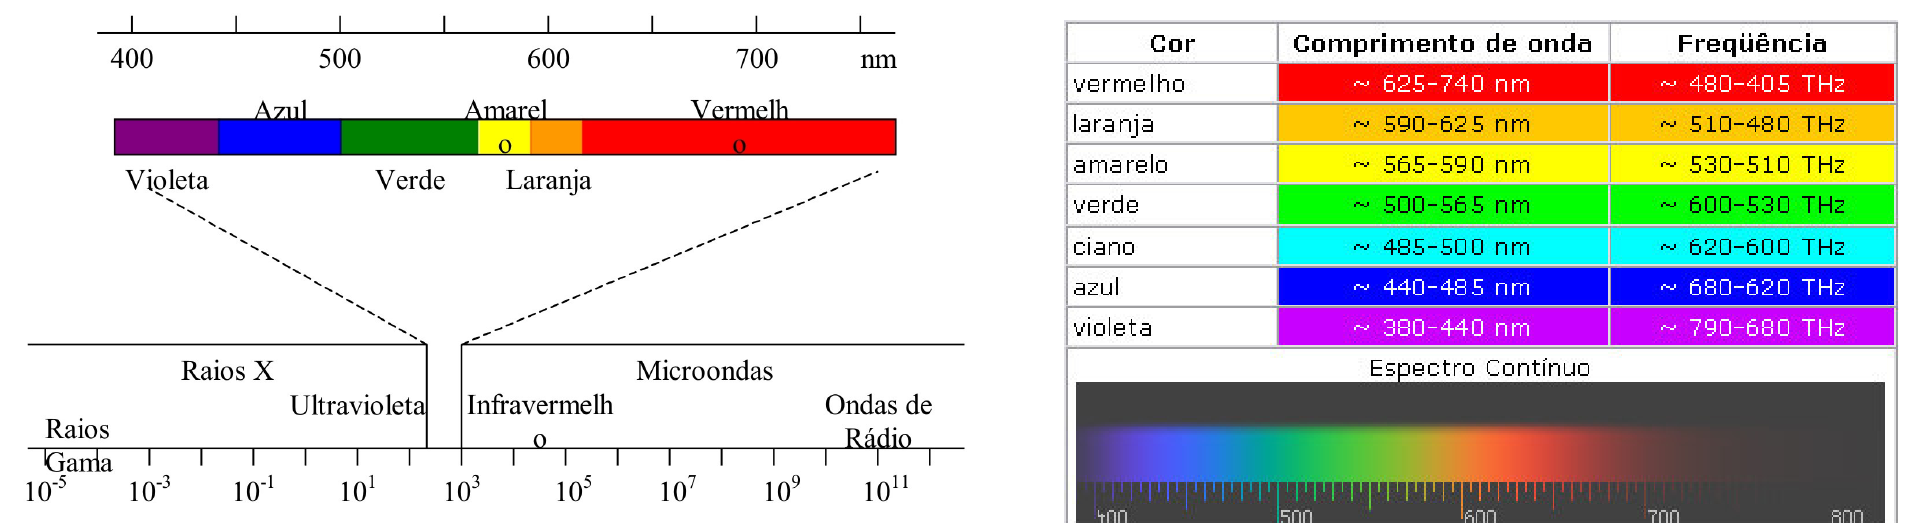
\includegraphics[width=.7\paperwidth]{figura1} %coloca a figura figura1 da pasta com largura 70 porcento da pagina
\caption{Espectro eletromagnético evidenciando a faixa de comprimentos de onda visíveis}
\label{fig:espectro}
\end{figure}
Vou citar a figura anterior, a figura \ref{fig:espectro}.
\chapter*{Discussão}
\addcontentsline{toc}{chapter}{Discussão}
Aqui vamos mostrar como citar seguindo as normas da ABNT \cite{NBR6023:2000}. Eu posso citar um livro, por exemplo \cite{livro1}.
As citações podem ser no formato alfanumérico ou somente numérico embora poucas pessoas acreditem nisso, como sugerido nas regras do relatório coloquei somente no formato alfanumérico\footnote{Exemplo de nota de rodapé}.
Caso você tenha qualquer dúvida sobre a bibliografia da ABNT consulte \cite{abntex}.




\chapter*{Conclusões}
\addcontentsline{toc}{chapter}{Conclusões}
É isso aí.

\bibliographystyle{abnt-alf}                                    %define estilo de bibliografia como abnt
\bibliography{Bibliografia}                                     %coloca bibliografia

\end{document}                                                  %finaliza documento
